\lecture{2009-10-21}

\subsection{Ungleichungen, Betrag-Kalkül-Teil}

\begin{definition}[Ungleichung]
Unter einer Ungleichung für reelle Zahlen $x,y$ verstehen wir einen Größenvergleich

  \begin{table}[h]
    \centering
    \begin{tabular}{|ll||ll|}
      \hline
      $x<y$ & "`kleiner"' & $x\leq y$ & "`kleiner gleich"' \\ 
      $x>y$ & "`größer"' & $x \geq y$ & "`größer gleich"' \\\hline
    \end{tabular}
  \end{table}
  
\end{definition}

\subsubsection*{Abschätzung}

"`$x<y$"' heißt Größe von $x$ durch Größe von $y$ abschätzen\\
Regelwerk für Abschätzungen (Anordnungsaxiome) $\leadsto$ Zahlengerade.

\begin{enumerate}
 \item $x \leq y, a\leq b \Rightarrow x+a \leq y+b$
 \item $x<y, 0 \leq a \Rightarrow ax \leq ay$
 
$x<y, 0 < a \Rightarrow ax < ay$
 \item $0<x\leq y \Rightarrow 0 < \frac{1}{y} \leq \frac{1}{x}$
\end{enumerate}

\begin{example}[Typische Aufgabe]
Lege $a$ fest mit Eigenschaft
\begin{align*}
-3a-2        &\leq 5 \leq -3a+4  &&\\
-3a-2        &\leq 5 & 5 &\leq -3a+4 \\
-3a          &\leq 7 & 1 &\leq -3a \\
-\frac{1}{3} &\leq a & a &\leq -\frac{7}{3}
\end{align*}

\end{example}

\begin{definition}[Obere Schranke]
$S \subset \mathbb{R}$ heißt nach oben beschränkt, falls eine Zahl $b$ existiert mit $S\subseteq \left]-\infty,b\right]$. $b$ heißt obere Schranke von $S$.
\end{definition}

\begin{definition}[Supremum]
Ist $S \subseteq \mathbb{R}$ nach oben beschränkt, so heißt die kleinste obere Schranke von $S$ das Supremum $s:=\sup S$.\\
(analog: \emph{Infimum} -- "`größte untere Schranke"' $u := \inf S$)
\end{definition}

\begin{note}Die kleinste obere Schranke muss nicht Element von $S$ sein, das \emph{Maximum} hingegen schon.\end{note}

\begin{example}
  \begin{itemize}
    \item $\sup \{x \in \mathbb{Q} | x^2 < 2 \} = \sqrt{2} \notin \mathbb{Q}$
    \item $\sup \{[a,b]\} = b \in [a,b]$
    \item $\inf \{ 1+\frac{1}{n}|n\in \mathbb{N}\} = 1$
  \end{itemize}
\end{example}

\begin{theorem}[Vollständigkeitsaxiom für $\mathbb{R}$]
Jede nach oben beschränkte Menge reeller Zahlen besitzt ein Supremum.
\end{theorem}

\begin{note}
$\mathbb{R}$ überabzählbar, $\mathbb{Q}$ abzählbar (siehe \cite[S. 11ff]{bornemann})
\end{note}

\begin{definition}[Betrag]
Betrag $|a|, a \in \mathbb{R}$\\
\[ |a| = 
\begin{cases}
 a & \text{ falls } a \geq 0 \\
 -a & \text{ falls } a < 0 \\
\end{cases}
\]
\end{definition}

\subsubsection*{Rechenregeln für Beträge}

\begin{enumerate}
 \item $-|a|\leq a \leq |a|$
 \item $|-a| = |a|$
 \item $|ab| = |a||b|$
 \item $\displaystyle\left|\frac{a}{b}\right| = \frac{|a|}{|b|}, b\neq 0$
\end{enumerate}

\subsubsection*{Anwendung: Dreiecksungleichung}
zu zeigen: $|a+b| \leq |a|+|b|$
\begin{proof}
  \begin{align*}
    -|a|&\leq a &\leq |a| \\
    -|b|&\leq b &\leq |b| \\
    \Rightarrow -(|a|+|b|)&\leq a+b &\leq |a|+|b| \\
    -(|a|+|b|)&\leq |a+b| &\leq |a|+|b|
  \end{align*}
\end{proof}

Abstandsmessung $|x-a| \leq \epsilon$\todo{unklar}

\subsubsection*{Rechenbeispiel}

\begin{example}
%%% Rechenbeispiel in der vorh. Version war offensichtlich falsch. Ich hab die Aufgabenstellung so
%%% angepasst, dass die Lösungsmenge nun korrekt sein sollte.
%%% --janosch
% $x\in \mathbb{R}$ gesucht mit $\frac{3}{x-9} \leq \frac{2}{x+2}$. Nenner $x\neq9 \land x\neq -2$
$x\in \mathbb{R}$ gesucht mit $\frac{3}{|x-9|} > \frac{2}{x+2}$. Nenner $x\neq9 \land x\neq -2$

\begin{center}
 \begin{tikzpicture}[line join=round,>=triangle 45,x=0.5cm,y=0.5cm]
  \draw[->,color=black] (-5,0) -- (15,0); % Linie+Pfeil des Zahlenstrahls
  \foreach \x in {-5,...,14}
  \draw[shift={(\x,0)},color=black] (0,0.2) -- (0,-0.2); % Zahlenmarkierungen
  \foreach \x in {-2,0,9}
  \draw[shift={(\x,0)},color=black] (0,0.3) -- (0,-0.3) node[below] {\footnotesize $\x$}; % Zahlen
  \draw [-(,ultra thick,color=orange] (-5,0) -- (-2,0); % Markierung links
  \draw [)-(,ultra thick,color=red](-2,0) -- (9,0); % Markierung mitte
  \draw [)-,ultra thick,color=purple] (9,0) -- (15,0); % Markierung rechts
 \end{tikzpicture}

\end{center}
\vspace{-.8cm}
\begin{align*}
\color{orange}M_1\color{black} &= \{x \in \mathbb{R} | x < -2\} \\
\color{red}M_2\color{black} &= \{x \in \mathbb{R} | -2 < x < 9\} \\
\color{purple}M_3\color{black} &= \{x \in \mathbb{R} | x > 9\}
\end{align*}

\begin{itemize}
 \item Diskussion von $M_1: x < -2$
\begin{align*}
|x-9|>0 &\Rightarrow \frac{3}{|x-9|} > 0 \\
x<-2 &\Rightarrow x+2<0 \Rightarrow \frac{2}{x+2}<0
\end{align*}
ganz $M_1$ zulässig
 \item Diskussion von $M_2: -2<x<9$
\begin{align*}
\Rightarrow x+2 &> 0 \\
x-9&<0 \Rightarrow |x-9|=9-x \\
\textrm{zu prüfen:} \\
\frac{3}{9-x} &> \frac{2}{x+2} \textrm{ (Betrag entfernt)} \\
3x+6 &> 18-2x \\
x &> \frac{12}{5} = 2 \frac{2}{5} \\
\end{align*}
erlaubt: $\frac{12}{5}<x<9$

 \item Diskussion von $M_3: x>9$
\begin{align*}
 \Rightarrow \overbrace{|x-9|}^{>0} = x-9 \\
\frac{3}{x-9} > \frac{2}{x+2} \\
\Rightarrow x>-24
\end{align*}
$M_3$ zulässig

Ergebnis: $\{x|x<-2, \frac{12}{5}<x<9, 9<x\}$
\end{itemize}

\end{example}

\subsubsection*{Anwendung: Geometrie}

\begin{itemize}

  \item Geradenschnitt

    \begin{center}
      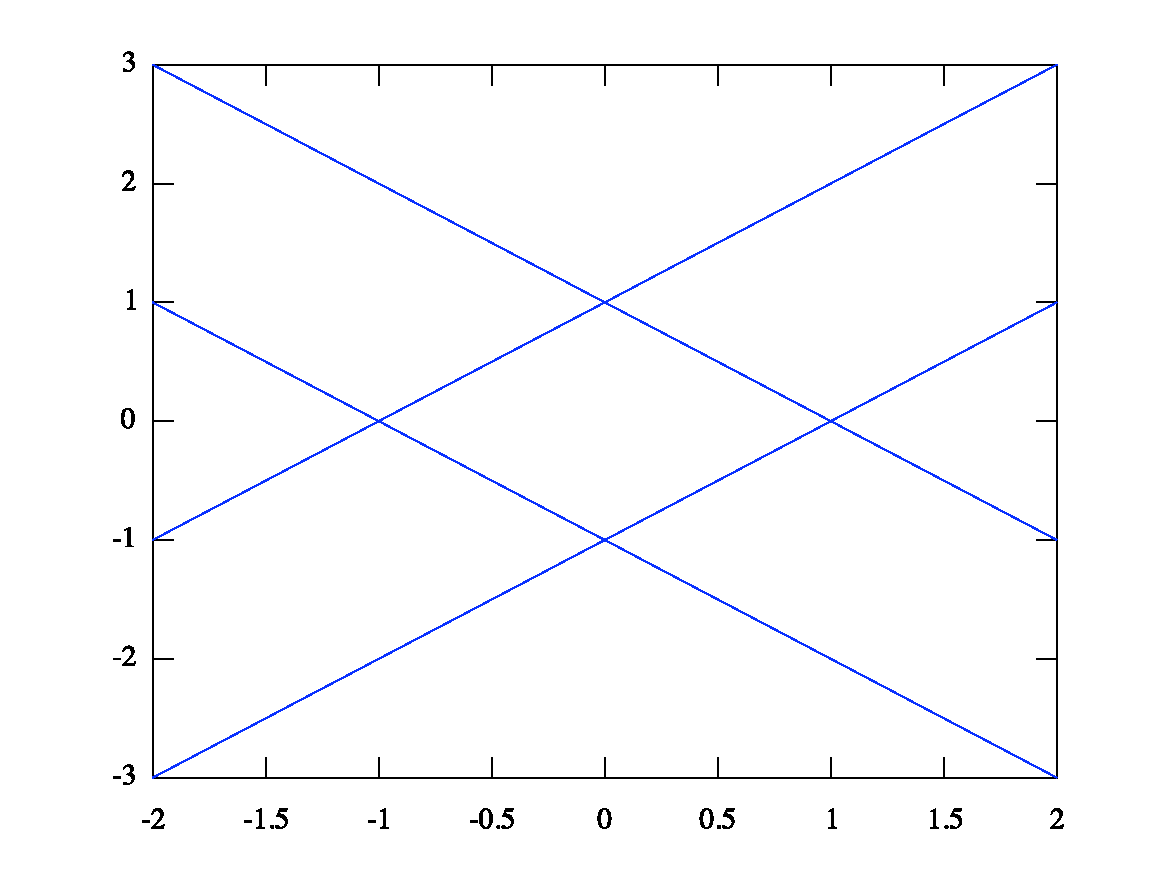
\includegraphics[width=0.8\textwidth]{include/geo_betraege.pdf}
      \captionof{figure}{geometrische Interpretation von $ |x|+|y| \leq 1$}
    \end{center}

    \begin{equation*}
    M = \{(x,y)\;|\; |x|+|y| \leq 1 \}; x,y \in \mathbb{R}
    \end{equation*}
    \begin{align*}
    |x|+|y| \leq 1 \Rightarrow &x \geq 0, y \geq 0: x+y \leq 1 \Rightarrow y \leq 1-x \\
            &x \geq 0, y < 0: x-y \leq 1 \Rightarrow y \geq -1+x \\
            &x < 0, y \geq 0: -x+y \leq 1 \Rightarrow y \leq 1+x \\
            &x < 0, y < 0: -x-y \leq 1 \Rightarrow y \geq -1-x \\
    \end{align*}
  
  \item
    Kreis um Ursprung mit Fläche\\
    Radius: $\{(x,y)| x^2+y^2\leq r^2 \}$\\
    Kreislinie: $\{(x,y)| x^2+y^2 = r^2 \}$
\end{itemize}
